\chapter{روش‌های پیشنهادی}

\section{معماری رمزگذار-رمزگشا}

در فصل پیشین، مرور کار‌های مرتبط، به توضیح مفاهیم پرداخته و به چندین مدل کارآمد در مسایل تقسیم‌بندی معنایی اشاره کردیم. بزرگ‌ترین اشکال استفاده از مدل های ذکر شده برای پردازش آنی، سرعت پایین آنها بوده که در استفاده برای خودرو‌های خودران چالش‌برانگیز می‌شود. در این فصل به طور مفصل به بررسی چندین مدل پیشنهادی برای تقسیم‌بندی معنایی که بخصوص برای پردازش آنی در خودرو‌های خودران طراحی شده اند می‌پردازیم.

\subsection{مدل \lr{SQNet}}

از راهکار های ساده برای بهبود عملکرد اکثر مدل های یادگیری عمیق که برای حل مسایل، افزایش اندازه شبکه است. این راهکار در حوزه تقسیم‌بندی معنایی نیز منجر به بوجود آمدن معماری های نوین مانند شبکه های مولد
\LTRfootnote{Generative Adversarial Networks (GAN)}
و مدل‌های انتشاری
\LTRfootnote{Diffusion Model}
شده است که به دلیل دقت بالا عموما در حوزه پزشکی مورد استفاده قرار می‌گیرند، اما به دلیل سرعت پایین آن‌ها در حوزه خودرو‌های خودران عملکرد خوبی از خود نشان نمی‌دهند. استفاده از این شبکه‌های دقیق اما بزرگ برای خودروهای خودران به‌طور کلی غیرقابل اجرا یا حداقل با دشواری و هزینه بسیار زیادی همراه است. پس تمرکز به سوی بهینه‌تر کردن مدل ها و استفاده از روش های نوین برای رسیدن به دقت مشابه و سرعت بیشتر تغییر کرده است، زیرا در خودرو‌های خودران قدرت پردازش و زمان کافی حائز اهمیت است. پس عمده مدل‌های معرفی شده به نوعی به معاوضه بین دقت و سرعت پرداخته و در تلاش هستند که با کمترین از دست رفت دقت بتوان سرعت پردازش را بالا برد.

تحقیقات گسترده ای بر روی کاهش توان پردازش مورد نیاز برای تقسیم‌بندی معنایی در خودرو‌های خودران صورت گرفته است. برای مثال معماری
\verb*|SqueezeNet|
\cite{iandola2016squeezenet}
نشان داد که با استفاده از یک معماری موثرتر که در آن از کانولوشن‌های تک واحدی برای فشرده کردن اطلاعات بکار گرفته شده، می‌توان همان دقت در پردازش تصاویر را با استفاده از ۵۰ برابر تعداد وزن‌های کمتر ایجاد نمود. همچنین با تغییر مولفه‌های جزئی‌تری مانند توابع ‌فعال‌ساز و یا حذف لایه‌هایی نظیر نرمال‌ساز می‌توانند در افزایش سرعت موثر باشند. مدل
\verb*|SQNet|
\cite{treml2016speeding}
که نیز از معماری رمزگذار-رمزگشا
\LTRfootnote{Encoder-Decoder Architecture}
استفاده می کند، توانسته است با استفاده از این‌گونه تغییرات به پردازش تقریبا آنی دست یابند.

معماری رمزگذار، مشابه آنچه در
\verb*|SqueezeNet|
آمده طراحی شده که ویژگی قابل توجه آن تعداد وزن‌های کمتر آن است که منجر به سرعت گرفتن پردازش آن می‌شود. بخش محاسباتی اصلی در این معماری آتش
\LTRfootnote{Fire module}
نامیده می‌شود که شامل سه عمل کانولوشن به همراه دو تابع‌فعال‌ساز می‌باشد. توابع‌فعال‌ساز یکسوساز
\LTRfootnote{Rectified linear unit (ReLU)}
با توابع‌فعال‌ساز واحد نمایی خطی
\LTRfootnote{Exponential linear unit (ELU)}
جایگزین شده‌اند که بار ‌محاسباتی کمتری داشته، و در عین حال اطلاعات منفی همچنان انتقال پیدا می‌کنند. در رمزگذار از هشت واحد آتش و سه لایه ادغام برای کاهش ابعاد تصویر استفاده شده است.

\begin{figure}[ht]
	\begin{subfigure}{\textwidth}
		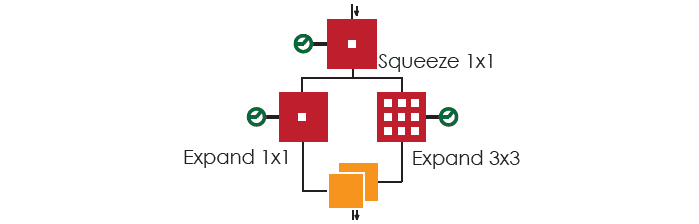
\includegraphics[width=\linewidth, height=0.2\textheight]{Images/Chapter3/SQNet_fire.png}
		\caption{واحد آتش}
		\label{f64}
	\end{subfigure}
	\begin{subfigure}{0.45\textwidth}
		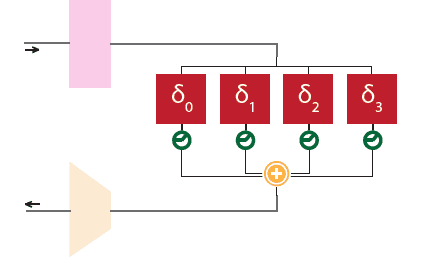
\includegraphics[width=\linewidth, height=0.2\textheight]{Images/Chapter3/SQNet_PDC.png}
		\caption{لایه کانولوشی موازی}
		\label{f65}
	\end{subfigure}
	\begin{subfigure}{0.45\textwidth}
		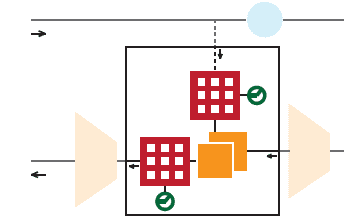
\includegraphics[width=\linewidth, height=0.2\textheight]{Images/Chapter3/SQNet_BRM.png}
		\caption{واحد تصحیح}
		\label{f65}
	\end{subfigure}
	\centering
	\caption{اجزاء معماری \lr{SQNet}}
	\label{fig:fig8}
\end{figure}

رمزگشا بر اساس یک لایه‌های
\verb*|parallel|
\verb*|dilated|
\verb*|convolutions|
مبتنی است که نقشه ویژگی‌ها را در خروجی رمزگذار در اندازه‌های میدان تاثیر مختلف ترکیب می‌کند. این واحد این کار را با استفاده از چهار کانولوشن با اندازه کرنل 3 انجام می‌دهد که معادل نمونه‌برداری لایه ورودی با نرخ‌های مختلف است. در نهایت خروجی چهار کانولوشن را با جمع زدن با یکدیگر با هم ادغام می‌کنیم که باعث می‌شود اندازه میدان دید در ورودی رمزگشا افزایش یابد. این کار باعث می‌شود نسبت به شبکه های تماما متصل، تعداد وزن‌های قابل توجه کمتری را داشته باشیم در حالی که عملکرد مدل حفظ می‌شود.

لایه‌های ادغامی داخل رمزگذار برای اطمینان از پایا بودن
\LTRfootnote{Translation Invariant}
در انتقالات استفاده می‌شوند. با این حال، این لایه‌ها به مرور زمان باعث کاهش وضوح تصویر می‌شوند، چراکه هر بار برخی از اطلاعات تصویر خلاصه یا حذف می‌شود. کانولوشن‌های معکوس
\LTRfootnote{Transposed Convolutions}
در رمزگشا برای افزایش ابعاد تصویر خارج شده از رمزگذار به اندازه اصلی استفاده می‌شوند. در حالت عادی، این معماری قدرت بازسازی بهینه‌ای نداشته و برخی اطلاعات تصویر اصلی از دست خواهد رفت که شدت آن به میزان استفاده از تعداد لایه های ادغامی و شدت کوچک‌نمایی تصویر دارد. برای کمرنگ‌تر کردن این مشکل، فقط از داده‌هایی که مستقیماً از لایه کانولوشن معکوس پیشین می‌آیند استفاده نمی‌کنیم، بلکه آن‌ها با دانش سطح پایین از لایه‌های زیرین رمزگذار ترکیب می‌شود. این کار به تشخیص ساختارهای با وضوح بالاتر کمک می‌کند که در تمیز کردن بهتر مرزهای اشیاء موثر است. پس از محاسبه کانولوشن‌های لایه فعلی و زیرین، هر دو ویژگی بدست آمده با یکدیگر ترکیب شده و سپس بزرگ‌نمایی می‌شود که به این واحد ها اصطلاحا واحد تصحیح
\LTRfootnote{Refinement Module}
گفته می‌شود. پیش‌تر اشاره شد که توابع‌فعال‌ساز متفاوتی برای رمزگذار استفاده می‌شود. این تابع‌ فعال‌ساز برای بخش رمزگشا نیز به همین نحو استفاده می‌شود.

\subsection{مدل \lr{ENet}}

معماری‌های متعددی برای حل مسایل تقسیم‌بندی معنایی مطرح شده‌اند که
\verb*|FCN|
و
\verb*|SegNet|
\cite{badrinarayanan2017segnet}
دو مدل مطرح در این حوزه هستند. از آنجایی که هر دو معماری بر اساس معماری پایه
\verb*|VGG|
طراحی شده‌اند، تعداد پارامتر‌ها و زمان استنتاج بالایی دارند و برای استفاده در حوزه‌هایی که نیاز به پردازش سریع و یا سخت‌افزار ضعیفی دارند مناسب نیستند. مدل
\verb*|ENet|
\cite{paszke2016enet}
\LTRfootnote{Efficient Neural Network}
با هدف پردازش سریع‌تر و دقت بالا طراحی شده است که نیز از معماری رمزگذار-رمزگشا استفاده می‌کند. 

معماری
\verb*|ENet|
از چندین بلوک تشکیل شده. بلوک ابتدایی
\LTRfootnote{Initial block}
شامل یک لایه ادغام حداکثری با پنجره‌‌های 2×2 بدون همپوشانی و یک لایه کانولوشنی با 13 فیلتر است که تصویر را به 16 نقشه ویژگی تبدیل می‌کند. هدف استفاده از این بلوک، کاهش ابعاد تصویر و تبدیل آن به بردار‌های ویژگی است تا اطلاعات غیرمرتبط تصویر حذف شده و بار محاسباتی کاهش پیدا کند. بلوک گلوگاه از اجزای کلیدی این معماری است که به طور مکرر در بخش های مختلف این معماری شاهد آن هستیم.

\begin{figure}[ht]
	\begin{subfigure}{0.45\textwidth}
		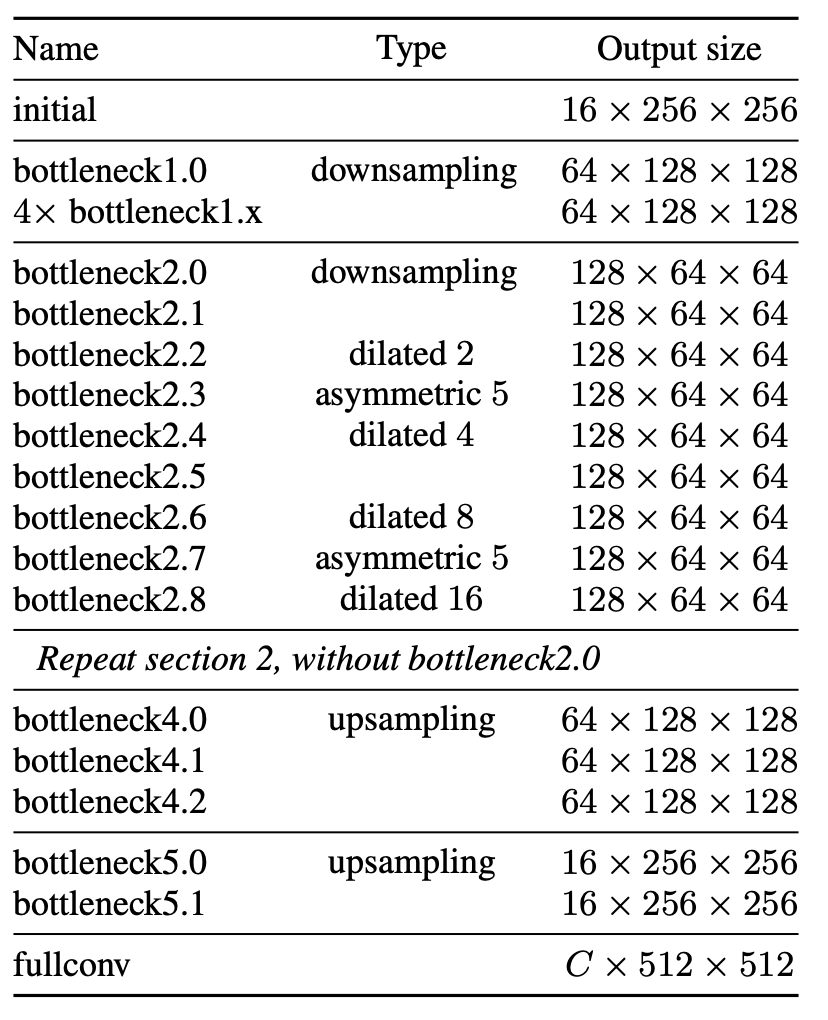
\includegraphics[width=\linewidth, height=0.3\textheight]{Images/Chapter3/ENet.png}
		\caption{معماری کلی شبکه \lr{ENet}}
		\label{f64}
	\end{subfigure}\hfil
	\begin{subfigure}{0.45\textwidth}
		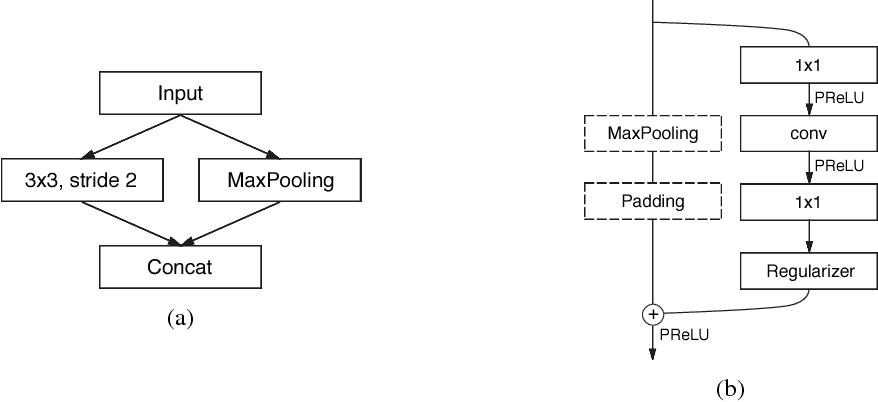
\includegraphics[width=\linewidth, height=0.2\textheight]{Images/Chapter3/ENet_blocks.png}
		\caption{معماری بلوک های شبکه \lr{ENet}}
		\label{f65}
	\end{subfigure}
	\centering
	\caption{نمونه تبدیل نقشه تقسیم‌بندی شده به تصویر رنگارنگ متناظر}
	\label{fig:fig7}
\end{figure}

نمونه‌برداری کاهشی
\LTRfootnote{Downsampling}
به طور کلی منجر به از دست رفتن برخی از اطلاعات داخل تصویر می‌شود و انجام آن بخصوص به صورت مکرر و با ضریب بزرگ به ضرر مدل است. اما از طرفی کاهش ابعاد تصویر به مصرف حافظه کمتر و کاهش بار محاسباتی و تعداد پارامتر های مدل کمک شایانی می‌کند. استراتژی استفاده شده در این معماری بدین گونه است که نمونه‌برداری کاهشی به کمترین تعداد ممکن و در ابتدای مدل انجام شود. مزیت انجام این‌کار در اول مسیر آن است که از پردازش تصاویر با ابعاد بزرگ که هزینه پردازش بالایی دارند جلوگیری می‌شود. برای سرعت بخشیدن به این فرآیند، عملیات ادغام به همراه یک کانولوشن به صورت موازی انجام شده و بردار‌های ویژگی حاصل با یکدیگر ترکیب می‌شوند.

بهینه سازی دیگر بر روی تابع‌فعالساز است. به گونه‌ای که در تمام مدل تابع فعالساز توابع‌فعال‌ساز یکسوساز پارامترسازي شده
\LTRfootnote{Parameterized ReLU (PReLU)}
جایگزین توابع‌فعال‌ساز یکسوساز شده است. این تابع‌فعالساز شیب منفی قابل آموزش دارد که به مدل انعطاف‌پذیری بیشتر و عملکرد بهتری داشته باشیم.

در آخر، استفاده از کانولوشن‌های گسترده
\LTRfootnote{Dilated convolutions}
نوعی دیگر از عملیات کانولوشن هستند که در آن‌ها فاصله‌ بین پیکسل‌های ورودی افزایش می‌یابد. در واقع، این نوع از کانولوشن‌ها به ورودی‌ها اعمال می‌شوند با استفاده از یک فیلتر کانولوشن با فضای پیکسل‌های بزرگ‌تر از یک باعث می‌شود اطلاعات بیشتری از ورودی‌ها در نظر گرفته شود. این نوع از کانولوشن‌ها معمولاً این امکان را برای شبکه فراهم می‌کنند تا بدون افزایش تعداد پارامترها میدان تاثیر بزرگ‌تری داشته باشد.

\section{معماری دو-شاخه}

\subsection{مدل \lr{Fast-SCNN}}

به مرور، تمایل به استفاده از معماری دو-شاخه
\LTRfootnote{Two-branch architecture}
در مدل‌های مطرح شده برای تقسیم‌بندی معنایی سریع افزایش یافته است؛ به طوری که دو شبکه با عمق های متفاوت بر روی تصویر با وضوح‌های متفاوت عمل کرده و در نهایت هر دو شاخه با یکدیگر ترکیب می‌شوند. این معماری اجازه می‌دهد تا در یک شاخه از شبکه‌ای عمیق
\LTRfootnote{Deep network}
بر روی تصویر با وضوح پایین استفاده شود تا اطلاعات اشیاء استخراج و آموخته شود و در شاخه دیگر شبکه‌ای کم عمق
\LTRfootnote{Shallow network}
بر روی همان تصویر اما با وضوح بالاتر به کار گرفته شود تا دقت نهایی تصویر خروجی بهبود یابد. از آنجایی که عمق شبکه و ابعاد تصویر اولیه به طور مستقیم بر روی سرعت پردازش تاثیرگذار هستند، معماری دو-شاخه بهینه‌سازی‌هایی برای پردازش سریع‌تر نسبت به معماری رمزگذار-رمزگشا دارد. مدل
\verb*|Fast|-\verb*|SCNN|
از ۴ بخش تقسیم شده که به صورت سری به یکدیگر متصل شده اند. در ادامه به معرفی اجزای مورد استفاده در این مدل می‌پردازیم.

\begin{figure}[ht]
	\centering
	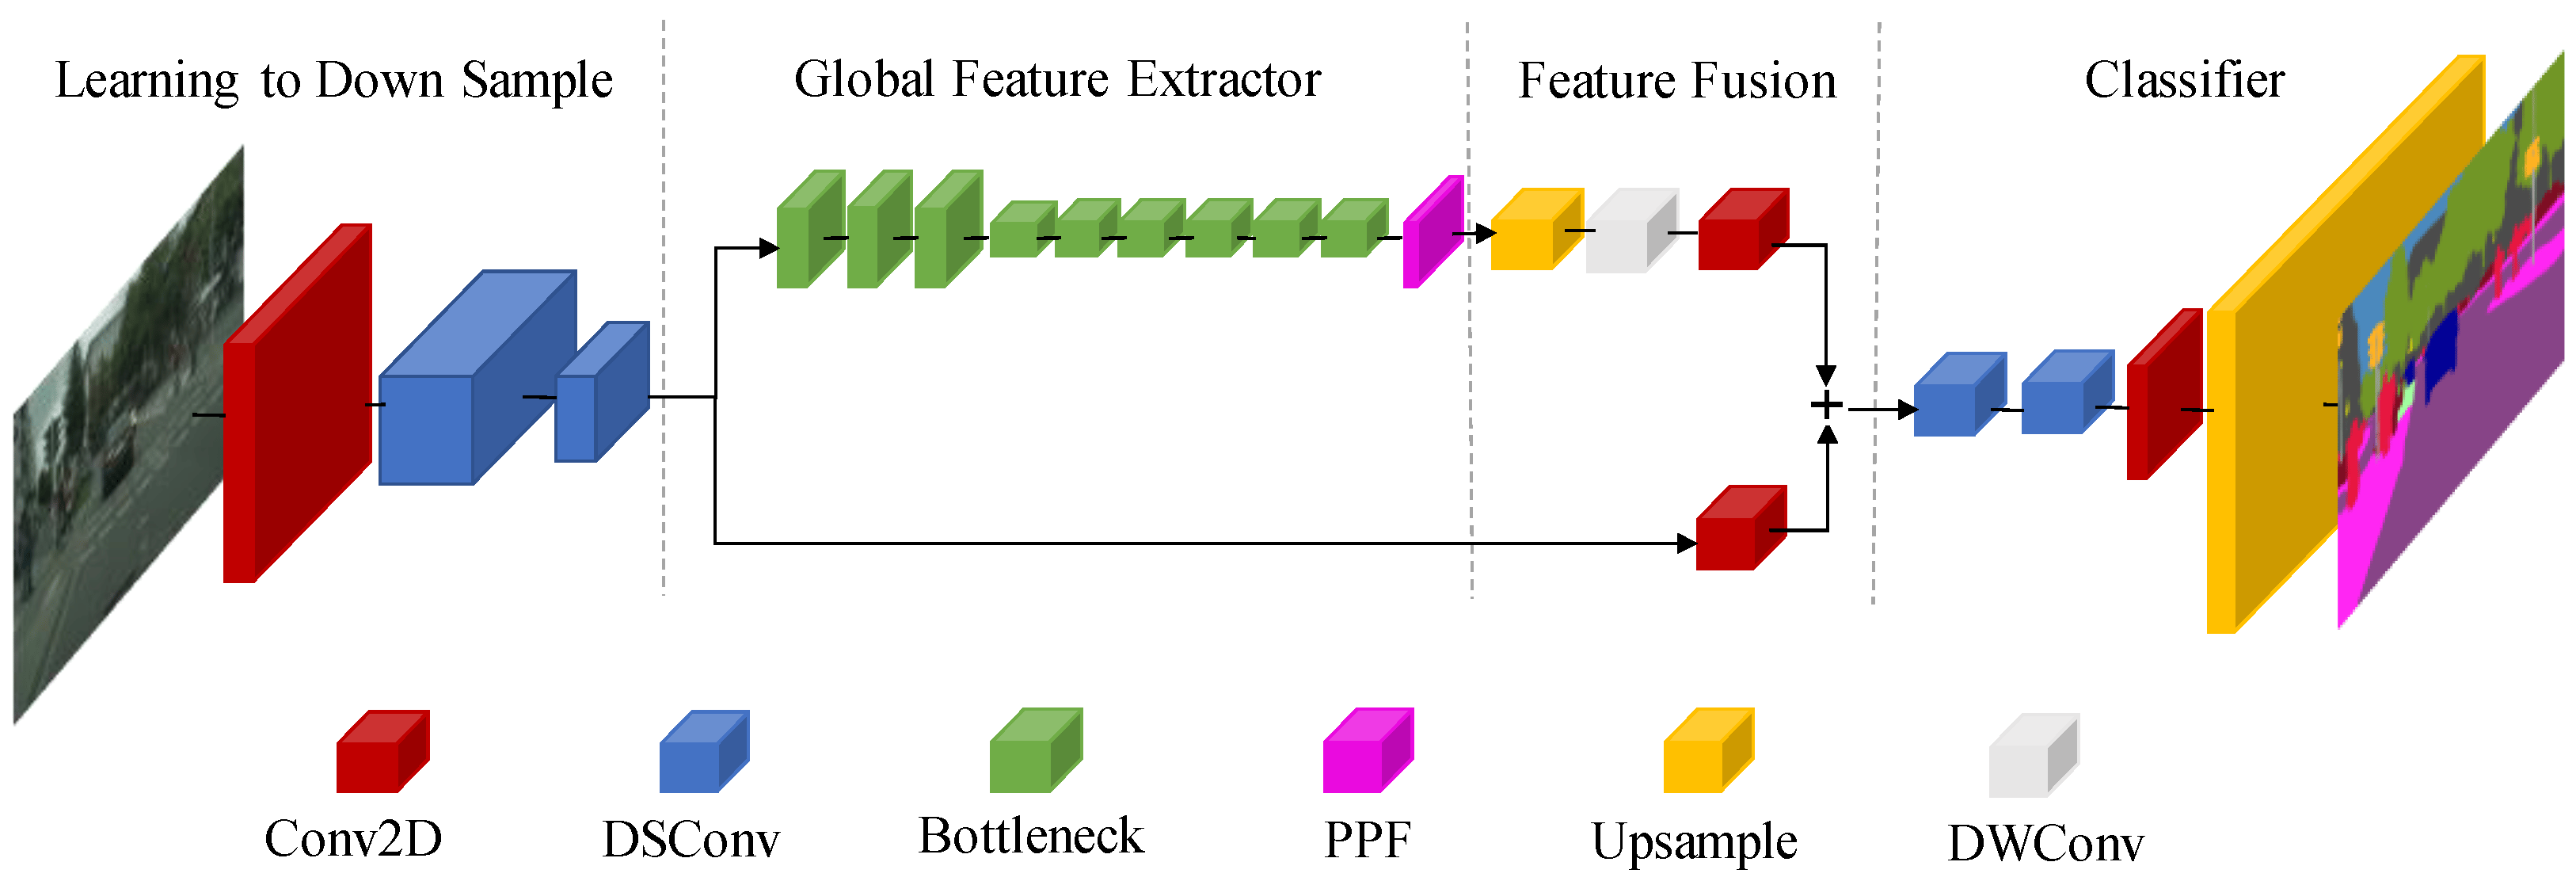
\includegraphics[width=0.9\linewidth, height=0.2\textheight]{Images/Chapter3/FastSCNN.png}
	\caption{معماری مدل \lr{Fast-SCNN}}
	\label{fig:fig10}
\end{figure}

\subsubsection{لایه‌ کانولوشنی تفکیک‌پذیر عمق‌محور}

در یک کانولوشن استاندارد بر روی تصاویر رنگی که عموما ۳ کانال رنگ دارند اینگونه انجام می‌شود که فیلتر به اندازه عمق رنگ ورودی اعمال شده و به ما امکان می‌دهد که کانال‌های رنگی را ترکیب کرده و آن‌ها را کم یا زیاد کنیم. به عبارتی اگر بخواهیم یک تصویر با ابعاد (۳،۱۲،۱۲) را به (۲۵۶،۸،۸) تبدیل کنیم به ۲۵۶ کرنل با ابعاد (۳،۵،۵) نیاز خواهیم داشت که در مجموع کمی بیش از یک میلیون عملیات ضرب خواهیم داشت.

در عملیات کانولوشنی عمق‌محور
\LTRfootnote{Depthwise Convolution}
، هر فیلتر به صورت جداگانه بر روی هر کانال اعمال شده و در نتیجه تعداد کانال‌های تصویر ثابت می‌ماند. به عبارتی، در تبدیل تصویر با ابعاد مشابه به ابعاد ثانوی (۳،۸،۸) نیاز به ۳ کرنل (به تعداد کانال‌های تصویر) با ابعاد (۱،۵،۵) داریم که در مجموع تقریبا ۵۰۰۰ عملیات ضرب می‌شود. سپس برای افزایش تعداد کانال‌های تصویر به عملیات کانولوشن نقطه‌محور
\LTRfootnote{Pointwise Convolution}
\cite{hua2018pointwise}
نیاز خواهیم داشت. برای مثال افزایش تعداد کانال‌های تصویر از ۳ به ۲۵۶ نیازمند ۲۵۶ کرنل با ابعاد (۳،۱،۱) دارد که در مجموع ۵۰۰۰۰ عملیات ضرب می‌شود. در نهایت ترکیب این دو لایه که لایه‌ کانولوشنی تفکیک‌پذیر عمق‌محور
\LTRfootnote{Depthwise Separable Convolutions}
\cite{chollet2017xception, nascimento2019dsconv}
نام دارد، معادل عملیات کانولوشن استاندارد می‌شود. لایه جدید در تئوری ۲۵ برابر و در عمل ۲ الی ۸ برابر سریع تر از کانولوشن استاندارد است.

\begin{figure}[ht]
	\centering
	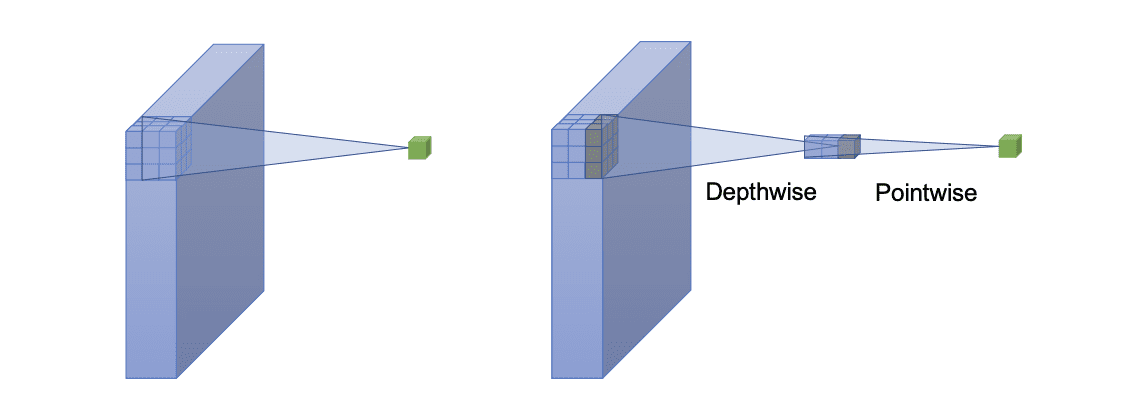
\includegraphics[width=0.9\linewidth, height=0.2\textheight]{Images/Chapter3/DepthwiseSeparableConvolution.png}
	\caption{مقایسه کانولوشن استاندارد و تفکیک‌پذیر عمق‌محور}
	\label{fig:fig9}
\end{figure}

\subsubsection{بخش \lr{learning to downsample}}

این اولین بخش از معماری
\verb*|Fast|-\verb*|SCNN|
است که از سه لایه اصلی تشکیل شده است که اولین آنها لایه کانولوشنی استاندارد است و دو جزء دیگر لایه‌های کانولوشنی تفکیک‌پذیر عمق‌محور که پیش‌تر معرفی شدند نام دارند. لایه‌های کانولوشنی تفکیک‌پذیر عمق‌محور در حالت عادی به لحاظ محاسباتی کارآمدتر هستند، اما برای اولین لایه از لایه کانولوشن استاندارد استفاده می‌کنیم زیرا برتری محاسباتی این لایه در اولین لایه به دلیل تنها ۳ کاناله بودن تصویر بیشتر است. پس از تمامی لایه‌های اصلی از نرمال‌سازی دسته‌ای و تابع‌فعال‌ساز
\verb*|ReLU|
استفاده شده است. معماری این بخش در شکل
\ref{fig:fig10}
قابل مشاهده است.

\subsubsection{بخش استخراج ویژگی‌های سراسری}

بخش استخراج ویژگی‌های سراسری
\LTRfootnote{Global feature extractor}
به دنبال استخراج اطلاعات از فضای تصویر برای تقسیم‌بندی است. تصویر ورودی این جزء، خروجی مستقیم بخش
\verb*|learning to downsample|
است که معادل یک هشتم ابعاد تصویر اصلی را دارد. این کوچک‌نمایی در عین کاهش میزان محاسبات، اکثر جزئیات مهم تصویر را حفظ می‌کند. در این بخش از تعدادی لایه بلوک اضافی گلوگاه
\LTRfootnote{Bottleneck residual block}
استفاده می‌شود که در آنها لایه کانولوشنی تفکیک‌پذیر عمقی جایگزین لایه‌های کانولوشنی عادی شده تا تعداد وزن‌های مورد استفاده در هر بلوک و در نتیجه تعداد عملیات برای محاسبه خروجی کاهش یابد. در آخر از لایه ادغام هرمی
\LTRfootnote{Pyramid pooling module (PPM)}
\cite{zhao2017pyramid}
استفاده شده که تا اطلاعات موجود در تصویر در مقیاس‌های مختلف تجمیع شوند که با استفاده از آنها پس از بلوک های اضافی گلوگاه تاثیر مثبتی بر روی خروجی می‌گذارد. نمای کلی این بخش در شکر 
\ref{fig:fig10}
قابل مشاهده است.

\subsubsection{گذاخت ویژگی‌ها و دسته‌بندی}

در بخش گداخت ویژگی‌ها
\LTRfootnote{Feature fusion module}
، از جمع ویژگی‌های به دلیل بهره‌وری بالای آن استفاده شده است. هرچند می‌توان از عملیات ترکیبی دیگر برای افزایش دقت استفاده کرد، در این معماری از جمع استفاده شده است. در بخش آخر به ترتیب از دو لایه
\verb*|DSConv|
و یک لایه
\verb*|Conv2D|
استفاده شد تا تصویر به اندازه اصلی برگردانده شود و در آخر از لایه
\verb*|softmax|
برای برگرداندن دسته‌بندی استفاده شد. به دلیل هزینه‌بر بودن محاسبات این تابع، می‌توان آن را با تابع
\verb*|argmax|
جایگزین کرد تا سرعت پردازش افزایش یابد.

\section{خلاصه}



